\ifdefined\COMPLETE
\else
    \input{./preambule-sacha-utf8.ltx}
    \begin{document}
\fi


\vspace*{-1.5cm}

\part{Les trinômes du second degré}

\section{Introduction}

\subsection{Rappel des années antérieures}

Résoudre les équations suivantes dans $\R$ :

\subsubsection{Exemple \no 1}

$x^2 - 9 = 0$ \\

Il faut factoriser. \\

\textbf{Rappel :} En troisième, on a appris trois identités remarquables : \\

\begin{itemize}
\item[•] $\left(a + b \right)^2 = a^2 + 2ab + b^2$ 
\item[•] $\left(a - b \right)^2 = a^2 - 2ab + b^2$ 
\item[•] $a^2 - b^2 = \left(a+b\right)\left(a-b\right)$ 
\end{itemize}

\vspace*{.3cm}

On a donc $x^2 - 9 = 0 \Longleftrightarrow \left(x+3\right)\left(x-3\right) = 0$. \\

\textbf{Rappel :} En troisième, on a appris si un produit est nul, au moins l'un de ses facteurs est nul. \\

\begin{tabular}{lll}
D'où $\left(x+3\right)\left(x-3\right) = 0$ & $ \Longleftrightarrow $ & $  x+3 = 0 $ ou $ x-3 = 0$ \\
& $\Longleftrightarrow$ & $x = -3 $ ou $x=3$ \\
\end{tabular}

Ainsi, $S = \lb -3 \; ; \; 3 \; \rb $

\subsubsection{Exemple \no 2}

\begin{tabular}{lll}
$ 9x^2 - 5 = 0$ & $\Longleftrightarrow$ & $\left(3x + \sqrt{5}\right)\left(3x - \sqrt{5}\right) = 0$ \\
& $\Longleftrightarrow$ & $3x + \sqrt{5} = 0 $ ou $3x - \sqrt{5} = 0$ \\
& $\Longleftrightarrow$ & $3x = -\sqrt{5}$ ou $3x = \sqrt{5}$ \\
& $\Longleftrightarrow$ & $x = \dfrac{-\sqrt{5}}{3} $ ou $x = \dfrac{\sqrt{5}}{3} $ \\
\end{tabular}

\vspace*{.3cm}

D'où $ S = \lb \dfrac{-\sqrt{5}}{3} \; ; \; \dfrac{\sqrt{5}}{3} \rb $

\subsubsection{Exemple \no 3}

\begin{tabular}{lll}
$x^2 - 14x + 49 = 0$ & $\Longleftrightarrow$ & $\left(x-7\right)^2 = 0 $\\
& $\Longleftrightarrow$ & $\left(x-7\right)\left(x-7\right) = 0$ \\
& $\Longleftrightarrow$ & $x-7 = 0$ ou $x-7 = 0$ \\
& $\Longleftrightarrow$ & $x = 7$ ou $x = 7$ \\
\end{tabular}

\vspace*{.3cm}

D'où $S = \lb 7 \rb $. \\

\textbf{N.B. :} Cet ensemble de solution est un \textbf{singleton}, bien que l'équation soit une équation du second degré. Cette solution est en fait une \textbf{solution double}.

\subsubsection{Exemple \no 4}

\begin{tabular}{lll}
$3x^2 - 2x\sqrt{21} + 7 = 0$ & $\Longleftrightarrow$ & $\left(x\sqrt{3} - \sqrt{7}\right)^2 = 0 $ \\
& $\Longleftrightarrow$ & $x\sqrt{3} - \sqrt{7} = 0$ \\
& $\Longleftrightarrow$ & $x\sqrt{3} = \sqrt{7}$ \\
& $\Longleftrightarrow$ & $ x = \dfrac{\sqrt{7}}{\sqrt{3}}$ \\
& $\Longleftrightarrow$ & $x = \dfrac{\sqrt{21}}{3}$ \\
\end{tabular}

D'où $ S = \lb \dfrac{\sqrt{21}}{3} \rb $

\subsubsection{Exemple \no 5}

\begin{tabular}{lll}
$x^2 + 36 = 0$ & $\Longleftrightarrow$ & $x^2 = -36$ \\
\end{tabular}

\vspace*{.3cm} 

Or, $\forall x \in \R, x^2 \geqslant 0$. \\

D'où $ S = \varnothing$ 

\subsubsection{Exemple \no 6}

\begin{tabular}{lll}
$17x^2 + 13 = 0 $ & $\Longleftrightarrow$ & $ 17x^2 = -13$ \\
\end{tabular}

\vspace*{.3cm}

Or, $\forall x \in \R, \forall a \in \R^+, ax^2 \geqslant 0$. \\

D'où $ S = \varnothing $

\subsection{Factoriser grâce à un « morceau » d'identité remarquable}

\subsubsection{Exemple \no 1}

\begin{tabular}{lll}
$x^2 + 6x - 7 = 0$ & $\Longleftrightarrow$ & $\left(x^2 + 6x + 9\right) - 16 = 0 $ \\
& $\Longleftrightarrow$ & $\left(x + 3\right)^2 - 4^2 = 0$ \\
& $\Longleftrightarrow$ & $\left(x + 3 + 4\right)\left(x + 3 - 4 \right) = 0 $ \\
& $\Longleftrightarrow$ & $\left(x + 7\right)\left(x - 1\right) = 0 $ \\
& $\Longleftrightarrow$ & $x + 7 = 0 $ ou $x - 1 = 0$ \\
& $\Longleftrightarrow$ & $ x = -7 $ ou $x = 1$ \\
\end{tabular}

\vspace*{.3cm}

D'où $S = \lb -7 \; ; \; 1 \rb$ 

\subsubsection{Exemple \no 2}

\begin{tabular}{lll}
$x^2 - 14x - 34 = 0 $ & $\Longleftrightarrow$ & $\left(x^2 - 14x + 49\right) - 81 = 0$ \\
& $\Longleftrightarrow$ & $\left(x-7\right)^2 - 9^2 = 0 $ \\
& $\Longleftrightarrow$ & $\left(x-7 + 9\right)\left(x-7 - 9\right) = 0$ \\
& $\Longleftrightarrow$ & $\left(x + 2\right)\left(x - 16\right) = 0$ \\
& $\Longleftrightarrow$ & $x + 2 = 0$ ou $x - 16 = 0$ \\
& $\Longleftrightarrow$ & $x = -2$ ou $x = 16$ \\
\end{tabular}

\vspace*{.3cm}

D'où $S = \lb -2 \; ; \; 16 \rb $ 

\subsubsection{Exemple \no 3}

\begin{tabular}{lll}
$x^2 - 5x + 4 = 0$ & $\Longleftrightarrow$ & $\left(x^2 - 5x + \dfrac{25}{4} \right) - \dfrac{9}{4} = 0$ \\
& $\Longleftrightarrow$ & $\left(x - \dfrac{5}{2}\right)^2 - \left(\dfrac{3}{2}\right)^2 = 0$ \\
& $\Longleftrightarrow$ & $\left(x - \dfrac{5}{2} + \dfrac{3}{2}\right)\left(x - \dfrac{5}{2} - \dfrac{3}{2} \right) = 0$ \\
& $\Longleftrightarrow$ & $\left(x-1\right)\left(x-4\right) = 0$ \\
& $\Longleftrightarrow$ & $ x -1 = 0$ ou $x - 4 = 0$ \\
& $\Longleftrightarrow$ & $ x = 1 $ ou $ x = 4 $ \\
\end{tabular}

\vspace*{.3cm}

D'où $S = \lb 1 \; ; \; 4 \rb $ 

\subsubsection{Exemple \no 4}

\begin{tabular}{lll}
$x^2 + 15x - 76 = 0 $ & $\Longleftrightarrow$ & $\left(x^2 + 15x + \dfrac{225}{4}\right) - \dfrac{529}{4} = 0$ \\
& $\Longleftrightarrow$ & $\left(x + \dfrac{15}{2}\right)^2 -  \left(\dfrac{23}{2}\right)^2 = 0$ \\
& $\Longleftrightarrow$ & $\left(x + \dfrac{15}{2} + \dfrac{23}{2}\right)\left(x + \dfrac{15}{2} - \dfrac{23}{2}\right) = 0$ \\
& $\Longleftrightarrow$ & $\left(x + 19\right)\left(x - 4\right) = 0$ \\
& $\Longleftrightarrow$ & $x + 19 = 0 $ ou $x - 4 = 0$ \\
& $\Longleftrightarrow$ & $x = -19 $ ou $x = 4$ \\
\end{tabular}

D'où $S = \lb -19 \; ; \; 4 \rb $ 

\subsubsection{Exemple \no 5}

\begin{tabular}{lll}
$9x^2 - 30x + 9 = 0$ & $\Longleftrightarrow$ & $\left(9x^2 - 30x +25\right) - 16 = 0 $ \\
& $\Longleftrightarrow$ & $\left(3x - 5\right)^2 - 4^2 = 0$ \\
& $\Longleftrightarrow$ & $\left(3x -5 + 4\right)\left(3x - 5 - 4\right) = 0$ \\
& $\Longleftrightarrow$ & $\left(3x -1\right)\left(3x - 9\right) = 0$ \\
& $\Longleftrightarrow$ & $ 3x - 1 = 0 $ ou $3x - 9 = 0$ \\
& $\Longleftrightarrow$ & $3x = 1 $ ou $3x = 9$ \\
& $ \Longleftrightarrow$ & $ x = \dfrac{1}{3} $ ou $x = 3$ \\
\end{tabular}

\vspace*{.3cm}

D'où $S = \lb \dfrac{1}{3} \; ; \; 3 \rb $ 

\subsubsection{Exemple \no 6}

\begin{tabular}{lll}
$36x^2 + 84x - 95 = 0 $ & $\Longleftrightarrow$ & $\left(36x^2 + 84x + 49\right) - 144 = 0 $ \\
& $\Longleftrightarrow$ & $\left(6x + 7\right)^2 - 12^2 = 0$ \\
& $\Longleftrightarrow$ & $\left(6x + 7 + 12\right)\left(6x + 7 - 12\right) = 0$ \\
& $\Longleftrightarrow$ & $\left(6x + 19\right)\left(6x -5\right) = 0$ \\
& $\Longleftrightarrow$ & $6x + 19 = 0$ ou $6x - 5 = 0$ \\
& $\Longleftrightarrow$ & $6x = -19$ ou $6x = 5$ \\
& $ \Longleftrightarrow$ & $x = \dfrac{-19}{6}$ ou $x = \dfrac{5}{6}$ \\
\end{tabular}

\vspace*{.3cm}

D'où $S = \lb \dfrac{-19}{6} \; ; \; \dfrac{5}{6} \rb $ 

\subsubsection{Exemple \no 7}

\begin{tabular}{lll}
$x^2 - 14x + 74 = 0$ & $\Longleftrightarrow$ & $\left(x^2 - 14x + 49\right) + 25 = 0$ \\
& $\Longleftrightarrow$ & $\left(x-7\right)^2 + 5^2 + 0$ \\
& $\Longleftrightarrow$ & $\left(x-7\right)^2 = -5^2 $ \\
\end{tabular}

Or $\forall x \in \R, x^2 \geqslant 0$. \\

D'où $S = \varnothing$ \\

\subsubsection{Exemple \no 8}

\begin{tabular}{lll}
$25x^2 + 20x + 53 = 0$ & $\Longleftrightarrow$ & $\left(25x^2 + 20x + 4\right) + 49 = 0$ \\
& $\Longleftrightarrow$ &  $\left(5x + 2\right)2 + 7^2 = 0$ \\
& $\Longleftrightarrow$ & $\left(5x + 2\right)^2 = -7^2$ \\
\end{tabular}

Or $\forall x \in \R, x^2 \geqslant 0$. \\

D'où $S = \varnothing$ 

\newpage

\section{Formules fondamentales}

\subsection{Résolutions, dans $\mathbf{\R}$, dans tous les types d'équations du second degré }

On peut écrire, pour $a$, $b$ et $c$ trois nombres réels avec $a \neq 0$, toutes les équations du second degré sous la forme : $ax^2 + bx + c = 0$. \\

\begin{tabular}{lll}
$ax^2 + bx + c = 0$ & $\Longleftrightarrow$ & $a\left(x^2 + \dfrac{b}{a}x + \dfrac{c}{a}\right) = 0$ \\
& $\Longleftrightarrow$ & $x^2 + \dfrac{b}{a}x + \dfrac{c}{a} = 0$ \\
& $\Longleftrightarrow$ & $ \left(x^2 + \dfrac{b}{a} x + \dfrac{b}{4a^2}\right) - \dfrac{b^2 - 4ac}{4a^2} = 0 $ \\
& $\Longleftrightarrow$ & $\left(x + \dfrac{b}{2a} \right)^2 - \dfrac{b^2 - 4ac}{\left(2a\right)^2} = 0$. \\
\end{tabular}

\vspace*{.3cm}

On a $\left(x + \dfrac{b}{2a}\right)^2 \geqslant 0$ et $\left(2a\right)^2 \geqslant 0$. \\

Notons alors $ \Delta = b^2 - 4ac$. \\

On a : $\left(x + \dfrac{b}{2a} \right)^2 - \dfrac{\Delta}{\left(2a\right)^2} = 0$ 

\begin{itemize}
\item[•] 1$^\mathrm{er}$ cas : $\Delta > 0$. \\

Si $\Delta > 0$, alors $\dfrac{\Delta}{\left(2a\right)^2} = \left(\dfrac{\sqrt{\Delta}}{2a}\right)^2$ \\


\begin{tabular}{lll}
Ainsi, on a : $\left(x + \dfrac{b}{2a} \right)^2 - \dfrac{\Delta}{\left(2a\right)^2} = 0$ & $\Longleftrightarrow$ & $\left(x + \dfrac{b}{2a} \right)^2 - \left(\dfrac{\sqrt{\Delta}}{2a}\right)^2 = 0 $ \\
& $\Longleftrightarrow$ & $\left(x + \dfrac{b}{2a} + \dfrac{\sqrt{\Delta}}{2a}\right)\left(x + \dfrac{b}{2a} - \dfrac{\sqrt{\Delta}}{2a}\right) = 0$ \\
& $\Longleftrightarrow$ & $ x + \dfrac{b + \sqrt{\Delta}}{2a} = 0 $ ou $x + \dfrac{b - \sqrt{\Delta}}{2a} = 0 $ \\
& $\Longleftrightarrow$ & $ x = -\dfrac{b + \sqrt{\Delta}}{2a}$ ou $x = \dfrac{b - \sqrt{\Delta}}{2a}$ \\
& $\Longleftrightarrow$ & $ x = \dfrac{-b - \sqrt{\Delta}}{2a}$ ou $x = \dfrac{-b + \sqrt{\Delta}}{2a}$ \\
\end{tabular}

\vspace*{.3cm}

D'où $ S = \lb \dfrac{-b - \sqrt{\Delta}}{2a} \; ; \; \dfrac{-b + \sqrt{\Delta}}{2a} \rb $. \\ 

On dit que le trinôme à \textbf{2 racines}. \\

\newpage

\item[•] 2$^\mathrm{ème}$ cas : $\Delta = 0$ \\

Si $\Delta = 0$, alors $\dfrac{\Delta}{\left(2a\right)^2} = 0$ \\

\begin{tabular}{lll}
Ainsi, on a : $\left(x + \dfrac{b}{2a} \right)^2 - \dfrac{\Delta}{\left(2a\right)^2} = 0$ & $\Longleftrightarrow$ & $\left(x + \dfrac{b}{2a} \right)^2  0$ \\
& $\Longleftrightarrow$ & $x + \dfrac{b}{2a} = 0$ \\
& $\Longleftrightarrow$ & $x = -\dfrac{b}{2a}$ \\
\end{tabular}

\vspace*{.3cm}

D'où $ S = \lb -\dfrac{b}{2a} \rb $. \\ 

On dit que le trinôme à une \textbf{racine double}. \\

\item[•]3$^\mathrm{ème}$ cas : $\Delta < 0$ \\

\begin{tabular}{lll}
Ainsi, on a : $\left(x + \dfrac{b}{2a} \right)^2 - \left(  \dfrac{\Delta}{\left(2a\right)^2}\right) = 0$ & $\Longleftrightarrow$ & $\left(x + \dfrac{b}{2a}\right)^2 = \dfrac{\Delta}{\left(2a\right)^2}$ \\
\end{tabular}

\vspace*{.3cm}

Or, $\Delta < 0$, donc $\dfrac{\Delta}{\left(2a\right)^2} < 0$. \\

Cependant, $\forall x \in \R, x^2 \geqslant 0$. \\

Ainsi, l'équation $\left(x + \dfrac{b}{2a}\right)^2 = \dfrac{\Delta}{\left(2a\right)^2}$ n'a pas de solution. \\

D'où $S = \varnothing$
\end{itemize}

\vspace*{.3cm}

\textbf{Récapitulatif} \\

$\forall a \in \R^*, \forall b \in \R, \forall c \in \R, ax^2 + bx + c = 0$ est un trinôme du second degré. \\

Soit $\Delta = b^2 - 4ac$ le discriminant de l'équation. \\

\begin{tabular}{lll}
Si $\Delta > 0$, alors le trinôme a deux racines, et $S = \lb \dfrac{-b - \sqrt{\Delta}}{2a} \; ; \; \dfrac{-b + \sqrt{\Delta}}{2a} \rb $ \\
Si $\Delta = 0$, alors le trinôme a une racine double, et $S = \lb -\dfrac{b}{2a} \rb $ \\
Si $\Delta < 0$, alors le trinôme n'a pas de racine réelle, et $ S = \varnothing$ \\
\end{tabular}

\newpage

\subsection{Exercices}

\subsubsection{Exemple \no 1}

$x^2 - 14x - 32 = 0$ \\

On a $a = 1$, $b = -14$, $c = -32$. \\

$ \Delta = b^2 - 4ac = 196 - 4 \times \left(-32\right) = 196 + 128 = 324 = 18^2$. \\

$\Delta > 0$, donc l'équation a deux solutions : \\

\begin{tabular}{lll}
$x_1 = \dfrac{-b - \sqrt{\Delta}}{2a}$ & ou & $x_2 = \dfrac{-b + \sqrt{\Delta}}{2a}$ \vspace*{.3cm} \\
$ x_1 = \dfrac{14 - 18}{2}$ & ou &$x_2 = \dfrac{14 + 18}{2}$ \vspace*{.3cm} \\
$x_1 = \dfrac{-4}{2}$ & ou & $x_2 = \dfrac{32}{2}$ \vspace*{.3cm} \\
$x_1 = -2$ & ou &$x_2 = 16$ \\
\end{tabular}

\vspace*{.3cm}

D'où $S = \lb -2 \; ; \; 16 \rb$. 

\subsubsection{Exemple \no 2}

$x^2 + 15x - 76 = 0$ \\

On a $a = 1$, $b = 15$, $c = -76$. \\

$ \Delta = b^2 - 4ac = 225 - 4 \times \left(-76\right) = 225 + 304 = 529 = 23^2$. \\

$\Delta > 0$, donc l'équation a deux solutions : \\

\begin{tabular}{lll}
$x_1 = \dfrac{-b - \sqrt{\Delta}}{2a}$ & ou & $x_2 = \dfrac{-b + \sqrt{\Delta}}{2a}$ \vspace*{.3cm} \\
$ x_1 = \dfrac{-15 - 23}{2}$ & ou &$x_2 = \dfrac{-15 + 23}{2}$ \vspace*{.3cm} \\
$x_1 = \dfrac{-38}{2}$ & ou & $x_2 = \dfrac{8}{2}$ \vspace*{.3cm} \\
$x_1 = -19$ & ou &$x_2 = 4$ \\
\end{tabular}

\vspace*{.3cm}

D'où $S = \lb -19 \; ; \; 4 \rb$. 

\newpage

\subsubsection{Exemple \no 3}

$36x^2 + 84x - 95 = 0$ \\

On a $a = 36$, $b = 84$ et $c = -95$. \\

$\Delta = b^2 - 4ac = 7056 - 4\left(36 \times \left(-95\right)\right) = 7056 + 13680 = 20 736 = 144^2$. \\

$\Delta > 0$, donc l'équation a deux solutions : \\

\begin{tabular}{lll}
$x_1 = \dfrac{-b - \sqrt{\Delta}}{2a}$ & ou & $x_2 = \dfrac{-b + \sqrt{\Delta}}{2a}$ \vspace*{.3cm} \\
$x_1 = \dfrac{-84 - 144}{72}$ & ou & $x_2 = \dfrac{-84 + 144}{72}$ \vspace*{.3cm} \\
$x_1 = \dfrac{-228}{72}$ & ou & $x_2 = \dfrac{60}{72}$ \vspace*{.3cm} \\
$x_1 = \dfrac{-19}{6}$ & ou & $x_2 = \dfrac{5}{6}$ \\
\end{tabular}

D'où $S = \lb -\dfrac{19}{6} \; ; \; \dfrac{5}{6} \rb $ 

\subsubsection{Exemple \no 4}

$25x^2 + 20x + 53$ \\

On a $a = 25$, $b = 20$, $c = 53$ \\

$ \Delta = b^2 - 4ac = 400 - 4 \times 25 \times 53 = 400 - 5 300 = -4 900$ \\

$\Delta < 0$, donc l'équation n'a pas de solution. \\

D'où $S = \varnothing$. 

\subsubsection{Exemple \no 5}

$127x^2 - 5x - 23 = 0$ \\

On a $a = 127$, $b = -5$, $c = -23$. \\

$ \Delta = b^2 - 4ac = 25 - 4 \times 127 \times \left(-23\right) = 25 + 11684 = 11 709$ \\

$\Delta > 0$, donc l'équation a deux solutions : 

\begin{tabular}{lll}
$x_1 = \dfrac{-b - \sqrt{\Delta}}{2a}$ & ou & $x_2 = \dfrac{-b + \sqrt{\Delta}}{2a}$ \vspace*{.3cm} \\
$ x_1 = \dfrac{5 - \sqrt{11709}}{254}$ & ou &$x_2 = \dfrac{5 + \sqrt{11709}}{254}$ \vspace*{.3cm} \\
\end{tabular}

D'où $S = \lb \dfrac{5 - \sqrt{11 709}}{254} \; ; \; \dfrac{5 + \sqrt{11 709}}{254} \rb$ 

\subsubsection{Exemple \no 6}

$1369x^2 - 4514x + 3721 = 0 $ \\

On a $a = 1 369$, $b = -4 514$, et $c = 3 721$. \\

$ \Delta = b^2 - 4ac = 20 376 196 - 20 376 196 = 0$ \\

$\Delta = 0$, donc l'équation a une solution : \\

$ x = -\dfrac{b}{2a} = \dfrac{4 514}{2 738} = \dfrac{61}{37}$. \\

$ S = \lb \dfrac{61}{37} \rb $ 

\subsubsection{Exemple \no 7}

$37 412x^2 -x + 29 = 0$ \\

On a $ a = 37 412$, $b = -1$ et $c = 29$. \\

$\Delta = b^2 - 4ac = 1 - 4 \times 29 \times 4 339 792 < 0$ \\

$\Delta < 0$, donc l'équation n'a pas de solution. \\

$S = \varnothing$ 

\newpage

\section{Forme canonique du trinôme}

\subsection{Rappels}

\begin{tabular}{lllll}
Soit une fonction $f$ : & $\R$ & $\longrightarrow$ & $\R$ & \\
& $x$ & $\longrightarrow$ & $f\left(x\right) = ax^2 + bx + c$, & avec $a \neq 0$ \\ 
\end{tabular}

On rappelle que $f\left(x\right)$ est un nombre réel, et que $f\left(x\right) = 0$ est l'\textbf{équation associée} à la fonction $f$. \\ De plus, la fonction $f$ est une \textbf{fonction polynôme du second degré}, ou une \textbf{fonction trinôme}. \\

\textbf{Exemple} \\

\begin{tabular}{llll}
Soit une fonction $f$ : & $\R$ & $\longrightarrow$ & $\R$ \\
& $x$ & $\longrightarrow$ & $f\left(x\right) = x^2 - 2x - 3$ \\ 
\end{tabular}

\vspace*{.3cm}

\begin{tikzpicture}[line cap=round,line join=round,>=triangle 45,x=1.0cm,y=1.0cm, scale=0.75]
\draw[->,color=black] (-6.27,0) -- (9.19,0);
\foreach \x in {-6,-5,-4,-3,-2,-1,1,2,3,4,5,6,7,8,9}
\draw[shift={(\x,0)},color=black] (0pt,2pt) -- (0pt,-2pt) node[below] {\footnotesize $\x$};
\draw[->,color=black] (0,-4.58) -- (0,7.98);
\foreach \y in {-4,-3,-2,-1,1,2,3,4,5,6,7}
\draw[shift={(0,\y)},color=black] (2pt,0pt) -- (-2pt,0pt) node[left] {\footnotesize $\y$};
\draw[color=black] (0pt,-10pt) node[right] {\footnotesize $0$};
\clip(-6.27,-4.58) rectangle (9.19,7.98);
\draw  plot (\x,{(\x)*(\x)-2*\x-3});
\begin{pgfonlayer}{background}   
\draw[step=1mm,ultra thin,AntiqueWhite!10] (-6.27,-4.58) grid (9.19,7.98);
\draw[step=5mm,very thin,AntiqueWhite!30]  (-6.27,-4.58) grid (9.19,7.98);
\draw[step=1cm,very thin,AntiqueWhite!50]  (-6.27,-4.58) grid (9.19,7.98);
\draw[step=5cm,thin,AntiqueWhite]          (-6.27,-4.58) grid (9.19,7.98);
\end{pgfonlayer} 
\end{tikzpicture}

\vspace*{.3cm}

Résolvons l'équation associée à la fonction $f$ :

\begin{tabular}{lll}
$\forall x \in \R, f\left(x\right) = 0$ & $\Longleftrightarrow$ & $x^2 - 2x - 3 = 0$ \vspace*{.3cm} \\
\end{tabular}

$\Delta = b^2 - 4ac = 4 - 4 \times \left(-3\right) = 4 + 12 = 16 = 4^2$ \\

$\Delta > 0$, donc l'équation a deux solutions : 

\begin{tabular}{lll}
$x_1 = \dfrac{-b - \sqrt{\Delta}}{2a}$ & ou & $x_2 = \dfrac{-b + \sqrt{\Delta}}{2a}$ \vspace*{.3cm} \\

$x_1 = \dfrac{2 - 4}{2}$ & ou & $x_2 = \dfrac{2 + 4}{2}$ \vspace*{.3cm} \\

$ x_1 = -1 $ & ou & $x_2 = 3$ \vspace*{.3cm} \\
\end{tabular} 

D'où $S = \lb -1 \; ; \; 3 \rb$. \\

Les solutions sont les abscisses des points d'intersection de la parabole et de l'axe des abscisses.

\newpage

\subsection{Généralisation de la factorisation des trinômes}

\begin{tabular}{lllll}
Soit une fonction $f$ : & $\R$ & $\longrightarrow$ & $\R$ & \\
& $x$ & $\longrightarrow$ & $f\left(x\right) = ax^2 + bx + c$, & avec $a \neq 0$ \\ 
\end{tabular}

\vspace*{.3cm}

Soient $\Delta$ le discriminant du trinôme, et $x_1$, $x_2$ ou $x_0$ ses racines éventuelles. \\

\begin{itemize}
\item[•] 1$^\mathrm{er}$ cas : $\Delta > 0$. \\

On a $ x_1 = \dfrac{-b - \sqrt{\Delta}}{2a}$ et $ x_2 = \dfrac{-b + \sqrt{\Delta}}{2a}$ \\

\begin{tabular}{lll}
$f\left(x\right)$ & $=$ & $ax^2 + bx + c$ \\
& $=$ & $a \left[\left(x + \dfrac{b}{2a}\right)^2 - \left(\dfrac{\sqrt{\Delta}}{2a}\right)^2 \right]$ \\
& $=$ & $a\left(x + \dfrac{b}{2a} + \dfrac{\sqrt{\Delta}}{2a} \right) \left(x + \dfrac{b}{2a} - \dfrac{\sqrt{\Delta}}{2a}\right)$ \\
& $=$ & $a\left(x + \dfrac{b + \sqrt{\Delta}}{2a} \right)\left(x + \dfrac{b - \sqrt{\Delta}}{2a} \right)$ \\
& $=$ & $a\left(x - \dfrac{-\left(b + \sqrt{\Delta}\right)}{2a} \right)\left(x - \dfrac{-\left(b - \sqrt{\Delta}\right)}{2a} \right)$ \\
& $=$ & $a\left(x - \dfrac{-b - \sqrt{\Delta}}{2a}\right)\left(x - \dfrac{-b + \sqrt{\Delta}}{2a}\right)$ \\
& $=$ & $a \left(x - x_1\right)\left(x - x_2\right)$ \\
\end{tabular}

\vspace*{.3cm}

\item[•]2$^\mathrm{ème}$ cas : $\Delta = 0$ \\

On a $x_0 = \dfrac{-b}{2a}$ \\

\begin{tabular}{lll}
$f\left(x\right)$ & $=$ & $ax^2 + bx + c$ \\
& $=$ & $a\left(x + \dfrac{b}{2a}\right)^2 $ \\
& $=$ & $a\left(x - \left(\dfrac{-b}{2a}\right)\right)^2 $ \\
& $=$ & $a\left(x-x_0\right)^2$ \\
\end{tabular}

\vspace*{.3cm}

\item[•]3$^\mathrm{ème}$ cas : $\Delta < 0$ \\

$f\left(x\right) = ax^2 + bx + c$ ne se factorise pas dans $\R$. \\

Mais, par l'absurde dans $\R$, on aurait :

\begin{tabular}{lll}
$f\left(x\right)$ & $=$ & $ax^2 + bx + c$ \\
& $=$ & $a\left(x - \alpha \right)\left(x - \beta\right)$
\end{tabular}

\vspace*{.3cm}

Et pour l'équation associée, on aurait : \\

\begin{tabular}{lll}
$f\left(x\right) = 0$ & $\Longleftrightarrow$ & $ax^2 + bx + c =0$ \\
& $\Longleftrightarrow$ & $a\left(x - \alpha \right)\left(x - \beta\right) = 0$ \\
& $\Longleftrightarrow$ & $x - \alpha = 0 $ ou $x - \beta = 0$ \\
& $\Longleftrightarrow$ & $ x = \alpha $ ou $x = \beta$ \\
\end{tabular}

\vspace*{.3cm}

On aurait donc deux solutions \textbf{non réelles}. 

\newpage

\textbf{Récapitulatif}

$\forall a \in \R^*, \forall b \in \R, \forall c \in \R, ax^2 + bx + c = 0$ est un trinôme du second degré. \\

Soit $\Delta = b^2 - 4ac$ le discriminant de l'équation. \\

\begin{itemize}
\item[•] Si $\Delta > 0$, alors $ax^2 + bx + c = a\left(x-x_1\right)\left(x-x_2\right)$ \\
\item[•] Si $\Delta = 0$, alors $ax^2 + bx + c = a\left(x-x_0\right)^2$\\
\item[•] Si $\Delta < 0$, alors $ax^2 + bx + c $ ne se factorise pas.
\end{itemize}
\end{itemize}

\subsection{Exercices}

\subsubsection{Exercice \no 1}

$f\left(x\right) = 5x^2 + 11x - 42$. Factoriser $f\left(x\right)$ \\

Après avec calculer $\Delta$, on trouve $ x_1 = \dfrac{-21}{5} $ et $x_2 = 2$ \\

\begin{tabular}{lll}
D'où $5x^2 + 11x - 42$ & $=$ & $5\left(x+\dfrac{21}{5}\right)\left(x-2\right)$ \\
& $=$ & $\left(5x+21\right)\left(x-2\right)$ \\
\end{tabular}

\subsubsection{Exercice \no 2}

$f\left(x\right) = 81x^2 - 72x + 16$. Factoriser $f\left(x\right)$ \\

Après avec calculer $\Delta$, on trouve $ x_0 = \dfrac{4}{9} $ \\

\begin{tabular}{lll}
D'où $81x^2 - 72x + 16$ & $=$ & $81\left(x-\dfrac{4}{9}\right)^2$ \\
& $=$ &  $9 \times 9 \times \left(x-\dfrac{4}{9}\right)
\left(x-\dfrac{4}{9}\right)$\\
& $=$ & $\left(9x - 4\right)\left(9x - 4\right)$ \\
& $=$ & $\left(9x - 4\right)^2$ \\
\end{tabular}

\subsubsection{Exercice \no 3}

$f\left(x\right) = 100x^2 + 3x + 7$. Factoriser $f\left(x\right)$ \\

On calcule $\Delta$, et on a $\Delta < 0$ \\

Donc $f\left(x\right)$ ne se factorise pas. 

\newpage

\vspace*{-2cm}

\subsection{Application : simplifier une fonction rationnelle}

\subsubsection{Application pour nourrissons déshydratés}

Simplifier la fonction rationnelle $f$, définie par :

\begin{tabular}{llll}
$f$ : & $\R$ & $\longrightarrow$ & $\R$ \\
& $x$ & $\longrightarrow$ & $f\left(x\right) = \dfrac{5x^2 - 18x - 8}{3x^2 - 13x + 7}$\\ 
\end{tabular}

$D_f = \lb x\in \R \; / \; 3x^2 - 13x + 7 \neq 0 \rb $ \\

Or, $3x^2 - 13x + 7 = 0 \Longleftrightarrow x = \dfrac{1}{3}$ ou $ x = 4$ \\

Donc $D_f = \R \setminus \lb \dfrac{1}{3} \; ; \; 4 \rb $ \\

Les solutions du trinôme $5x^2 - 18x - 8$ sont $x_1 = -\dfrac{2}{5}$ et $x_2 = 4$. \\

Les solutions du trinôme $3x^2 - 13x + 7$ sont $x_1 = -\dfrac{1}{3}$ et $x_2 = 4$. \\

\begin{tabular}{lll}
Ainsi, $\forall x \in D_f, f\left(x\right)$ & $=$ &$ \dfrac{5\left(x + \dfrac{2}{5}\right)\left(x-4\right)}{3\left(x-\dfrac{1}{3}\right)\left(x-4\right)}$ \\
& $=$ & $\dfrac{5\left(x + \dfrac{2}{5}\right)}{3\left(x-\dfrac{1}{3}\right)}$ \\
& $=$ & $\dfrac{5x + 2}{3x - 1}$ \\
\end{tabular}

\subsubsection{Application pour élèves musclés}

\begin{tabular}{llll}
Soit une fonction $f$ : & $\R$ & $\longrightarrow$ & $\R$ \\
& $x$ & $\longrightarrow$ & $f\left(x\right) = \dfrac{253x^2 - 344x - 1349}{391x^2 - 1506x + 923}$\\ 
\end{tabular}

$D_f = \lb x\\in \R \; / \; 391x^2 - 1506x + 923 \neq 0 \rb $ \\

Or, $391x^2 - 1506x + 923 = 0 \Longleftrightarrow x = \dfrac{13}{17}$ ou $ x = \dfrac{71}{23}$ \\

Donc $D_f = \R \setminus \lb \dfrac{13}{17} \; ; \; \dfrac{71}{23} \rb $ \\

Les solutions du trinôme $253x^2 - 344x - 1349$ sont $x_1 = \dfrac{-19}{11}$ et $x_2 = \dfrac{71}{23}$. \\

Les solutions du trinôme $391x^2 - 1506x + 923$ sont $x_1 = \dfrac{13}{17}$ et $x_2 = \dfrac{71}{23}$.

\begin{tabular}{lll}
Ainsi, $\forall x \in D_f, f\left(x\right)$ & $=$ &$ \dfrac{2535\left(x + \dfrac{19}{11}\right)\left(x-\dfrac{71}{23}\right)}{3\left(x-\dfrac{13}{17}\right)\left(x-\dfrac{71}{23}\right)}$ \\
& $=$ &$ \dfrac{2535\left(x + \dfrac{19}{11}\right)}{3\left(x-\dfrac{13}{17}\right)}$ \\
& $=$ & $\dfrac{11x + 19}{17x - 13}$ \\
\end{tabular}

\vspace*{-5cm}

\newpage

\section{Signe du trinôme}

\subsection{Introduction et rappel}

\subsubsection{Introduction}

\begin{tabular}{lllll}
Soit une fonction $f$ : & $\R$ & $\longrightarrow$ & $\R$ & \\
& $x$ & $\longrightarrow$ & $f\left(x\right) = ax^2 + bx + c$, & avec $a \neq 0$ \\ 
\end{tabular}

\vspace*{.3cm}

Soit $f\left(x\right) = 0$ l'équation associée à la fonction $f$. \\ Soient $\Delta$ son discriminant, et $x_1$, $x_2$, et $x_0$ les racines éventuelles du trinôme. \\

On pose pour tout ce paragraphe $x_1 < x_2$.

\subsubsection{Rappel : les tableaux de signes }

Soit $f\left(x\right) = \left(2x+6\right)\left(-3x+12\right)$. On a donc $x_1 = -3$ et $x_2 = 4$ \\

\begin{tikzpicture}
\tkzTabInit[lgt=3.2,espcl=2]
{ $x$  /1,
$2x+6$   /1,
$-3x + 12$ /1,
$\left(2x+6\right)\left(-3x+12\right)$ /1}
{$ - \infty $ , $-3 $ , $4 $ , $ + \infty $}
\tkzTabLine{ , - , z , +, t  ,+  }
\tkzTabLine{ , + , t , + , z, - }
\tkzTabLine{ , - , z , +, z, - }
\end{tikzpicture}

\subsection{Cas généraux}

\subsubsection{Premier cas : $\mathbf{\Delta > 0}$}

Si $\Delta > 0$, alors $f\left(x\right) = a\left(x-x_1\right)\left(x-x_2\right)$ \\

\begin{tikzpicture}
\tkzTabInit[lgt=4.2,espcl=3]
{ $x$  /1,
$x-x_1$   /1,
$x-x_2$   /1,
$\left(x-x_1\right)\left(x-x_2\right)$ /1,
$a\left(x-x_1\right)\left(x-x_2\right)$ /1}
{$ - \infty $ , $x_1 $ , $x_2 $ , $ + \infty $}
\tkzTabLine{ , - , z , +, t, +  }
\tkzTabLine{ , - , t , - , z, + }
\tkzTabLine{ , + , z , -, z, + }
\tkzTabLine{ , $Signe de $a$ $, z , $Signe de $-a$ $ , z, $Signe de $a$ $ }
\end{tikzpicture}

\newpage

\subsubsection{Deuxième cas : $\mathbf{\Delta = 0}$}

Si $\Delta = 0$, alors $f\left(x\right) = a\left(x-x_0\right)^2 = a\left(x-x_0\right)\left(x-x_0\right)$ \\

\begin{tikzpicture}
\tkzTabInit[lgt=4.2,espcl=3]
{ $x$  /1,
$x-x_0$   /1,
$x-x_0$   /1,
$\left(x-x_0\right)^2$ /1,
$a\left(x-x_0\right)^2$ /1}
{$ - \infty $ , $x_0 $ , $ + \infty $}
\tkzTabLine{ , - , z , +  }
\tkzTabLine{ , - , z, + }
\tkzTabLine{ , + , z , + }
\tkzTabLine{ , $Signe de $a$ $, z , $Signe de $a$ $ }
\end{tikzpicture}

\vspace*{.3cm}

\subsubsection{Troisième cas : $\mathbf{\Delta < 0}$}

Si $\Delta < 0$, alors $f\left(x\right)$ ne se factorise pas.  \\

\begin{tabular}{lll}
On a cependant $f\left(x\right)$ & $ = $ & $ a\left[\left(x+ \dfrac{b}{2a}\right)^2 - \dfrac{\Delta}{4a^2}\right]$ \\
& $=$ & $a\left[\left(x+\dfrac{b}{2a}\right) + \dfrac{-\Delta}{4a^2}\right]$ \\
\end{tabular}

\vspace*{.3cm}

On a $\Delta <0$, d'où $-\Delta > 0$ et $-\dfrac{\Delta}{4a^2} > 0$ \\

De plus, $\forall x \in \R, x^2 \geqslant 0$, d'où $\left(x+\dfrac{b}{2a}\right)^2 \geqslant 0$. \\

Ainsi, on a $\left(x+\dfrac{b}{2a}\right) + \dfrac{-\Delta}{4a^2} > 0$. \\

Le signe de $f\left(x\right) = a\left[\left(x+\dfrac{b}{2a}\right) + \dfrac{-\Delta}{4a^2}\right] $ dépend donc du signe de $a$. On peut écrire : \\

\begin{tikzpicture}
\tkzTabInit[lgt=4.2,espcl=3]
{ $x$  /1,
$f\left(x\right)$ /1}
{$ - \infty $ , $ + \infty $}
\tkzTabLine{ , $Signe de $a$ $ }
\end{tikzpicture}

\newpage

\subsubsection{Récapitulatif}

$\forall a \in \R^*, \forall b \in \R, \forall c \in \R, ax^2 + bx + c = 0$ est un trinôme du second degré. On note $f\left(x\right) = ax^2 + bx + c$. On peut connaître le signe de ce trinôme en fonction du signe de son discriminant :

\begin{itemize}
\item[•] 1$^\mathrm{er}$ cas : Si $\Delta > 0$ \\

\begin{tikzpicture}
\tkzTabInit[lgt=4.2,espcl=3]
{ $x$  /1,
$f\left(x\right)$ /1}
{$ - \infty $ , $x_1$, $x_2$,  $ + \infty $}
\tkzTabLine{ , $Signe de $a$ $, z, $Signe de $-a$ $, z, $Signe de $a$ $ }
\end{tikzpicture}

\item[•] 2$^\mathrm{ème}$ cas : Si $\Delta = 0$ \\

\begin{tikzpicture}
\tkzTabInit[lgt=4.2,espcl=3]
{ $x$  /1,
$f\left(x\right)$ /1}
{$ - \infty $ , $x_0$,  $ + \infty $}
\tkzTabLine{ , $Signe de $a$ $, z, $Signe de $a$ $ }
\end{tikzpicture}

\item[•] 3$^\mathrm{ème}$ cas : Si $\Delta < 0$ \\

\begin{tikzpicture}
\tkzTabInit[lgt=4.2,espcl=3]
{ $x$  /1,
$f\left(x\right)$ /1}
{$ - \infty $ , $ + \infty $}
\tkzTabLine{ , $Signe de $a$ $ }
\end{tikzpicture}
\end{itemize}

\subsection{Exercices}

\subsubsection{Exercice \no 1}

$3x^2 + 5x - 8 \leqslant 0$ \\

On étudie le trinôme $3x^2 + 5x - 8$. Son discriminant est positif, et ses racines sont $x_1 = \dfrac{-8}{3}$ et $x_2 = 1$. \\

$a = 3 > 0$, d'où : \\

\begin{tikzpicture}
\tkzTabInit[lgt=4.2,espcl=3]
{ $x$  /1,
$3x^2 + 5x - 8$ /1}
{$ - \infty $ , $\dfrac{-8}{3}$, $1$, $+ \infty $}
\tkzTabLine{ , +, z, -, z, + }
\end{tikzpicture}

\vspace*{.3cm}

$S = \left[-\dfrac{8}{3} \; ; \; 1 \right]$ \\

De même, on a aussi : \\

\begin{tabular}{ll}
$3x^2 + 5x - 8 < 0$ & $S = \left]\dfrac{-8}{3} \; ; \; 1\right[$ \\
$3x^2 + 5x - 8 \geqslant 0$ & $S = \left]-\infty \; ; \; \dfrac{-8}{3} \right] \cup \left[1 \; ; \; + \infty \right[$ \\
$3x^2 + 5x - 8 \geqslant 0$ & $S = \left]-\infty \; ; \; \dfrac{-8}{3} \right[ \cup \left]1 \; ; \; + \infty \right[$ \\
\end{tabular}

\subsubsection{Exercice \no 2}

$25x^2 -30x +9 \leqslant 0$ \\

On étudie le trinôme $25x^2 -30x +9$. Son discriminant est nul, et sa racine est $x_0 = \dfrac{3}{5}$. \\

$a = 25 > 0$, d'où : \\

\begin{tikzpicture}
\tkzTabInit[lgt=4.2,espcl=3]
{ $x$  /1,
$25x^2 -30x +9$ /1}
{$ - \infty $ , $\dfrac{3}{5}$, $+ \infty $}
\tkzTabLine{ , +, z, + }
\end{tikzpicture}

\vspace*{.3cm}

$S = \lb \; \dfrac{3}{5} \; \rb $ \\

De même, on a aussi : \\

\begin{tabular}{ll}
$25x^2 -30x +9 < 0$ & $S = \varnothing $ \\
$25x^2 -30x +9 \geqslant 0$ & $S = \left]-\infty \; ; \; + \infty \right[$ \\
$25x^2 -30x +9 \geqslant 0$ & $S = \left]-\infty \; ; \; \dfrac{3}{5} \right[ \cup \left]\dfrac{3}{5} \; ; \; + \infty \right[$ \\
\end{tabular}

\subsubsection{Exercice \no 3}

$12x^2 -5x +10 \leqslant 0$ \\

On étudie le trinôme $12x^2 -5x +10$. Son discriminant est nul. Il est donc du signe de $a$ pour tout réel $x$. \\

$a = 12 > 0$, d'où : \\

\begin{tikzpicture}
\tkzTabInit[lgt=4.2,espcl=3]
{ $x$  /1,
$12x^2 -5x +10$ /1}
{$ - \infty $ ,  $+ \infty $}
\tkzTabLine{ , + }
\end{tikzpicture}

\vspace*{.3cm}

$S = \varnothing $ \\

De même, on a aussi : \\

\begin{tabular}{ll}
$12x^2 -5x +10 < 0$ & $S = \varnothing $ \\
$12x^2 -5x +10 \geqslant 0$ & $S = \left]-\infty \; ; \; + \infty \right[$ \\
$12x^2 -5x +10 \geqslant 0$ & $S = \left]-\infty \; ; \; + \infty \right[$ \\
\end{tabular}

\newpage

\subsubsection{Exercice \no 4, un peu plus musclé}

Résoudre l'inéquation : \\

$\left(5x^2 +8x +3\right)\left(-7x^2 -2x + 9\right) \leqslant 0$ \\

On étudie le trinôme $5x^2 +8x +3$. Son discriminant est positif, et ses racines sons $x_1 = -1$ et $x_2 = \dfrac{-3}{5}$. \\

On étudie le trinôme $-7x^2 -2x + 9$. Son discriminant est positif, et ses racines sons $x_1 = 1$ et $x_2 = \dfrac{-9}{7}$. \\

D'où : \\

\begin{tikzpicture}
\tkzTabInit[lgt=5,espcl=2]
{ $x$               /1,
$5x^2 +8x +3$       /1,
$-7x^2 -2x + 9$     /1,
$\left(5x^2 +8x +3\right)\left(-7x^2 -2x + 9\right)$     /1}
{$ - \infty $ , $\dfrac{-9}{7}$, $-1$, $\dfrac{-3}{5}$, $1$, $+ \infty $}
\tkzTabLine{ , + , t , + , z , - , z , + , t , + }
\tkzTabLine{ , - , z , + , t , + , t , + , z , - }
\tkzTabLine{ , - , z , + , z , - , z , + , z , - }
\end{tikzpicture}

\vspace*{.3cm}

$S = \left]-\infty \; ; \; \dfrac{-9}{7}\right]\cup\left[-1 \; ; \; \dfrac{-3}{5}\right]\cup \left[1 \; ; \; +\infty\right[ $ 

\subsubsection{Exercice \no 5}

Résoudre l'inéquation :\\

$\dfrac{5x^2 + 8x + 3}{-7x^2 - 2x + 9} \leqslant 0$ \\

Il ne faut pas que $-7x^2 - 2x + 9 = 0$. Donc il ne faut pas que $x = -\dfrac{9}{7}$ ou que $x = 1$. \\

D'après l'exercice précédent, on peut dresser le tableau de signes suivant : \\

\begin{tikzpicture}
\tkzTabInit[lgt=5,espcl=2]
{ $x$               /1,
$5x^2 +8x +3$       /1,
$-7x^2 -2x + 9$     /1,
$\left(5x^2 +8x +3\right)\left(-7x^2 -2x + 9\right)$     /1}
{$ - \infty $ , $\dfrac{-9}{7}$, $-1$, $\dfrac{-3}{5}$, $1$, $+ \infty $}
\tkzTabLine{ , + , t , + , z , - , z , + , t , + }
\tkzTabLine{ , - , z , + , t , + , t , + , z , - }
\tkzTabLine{ , - , d , + , z , - , z , + , d , - }
\end{tikzpicture}

\vspace*{.3cm}

$S = \left]-\infty \; ; \; \dfrac{-9}{7}\right[\cup\left[-1 \; ; \; \dfrac{-3}{5}\right]\cup \left]1 \; ; \; +\infty\right[ $ 

\newpage

\section{Interprétation géométrique}

\begin{tabular}{llll}
Soit une fonction $f$ : & $\R$ & $\longrightarrow$ & $\R$ \\
& $x$ & $\longrightarrow$ & $f\left(x\right) = -x^2 + 4x + 5$ \\ 
\end{tabular}

\vspace*{.3cm}

\begin{tabular}{llll}
Soit une fonction $g$ : & $\R$ & $\longrightarrow$ & $\R$ \\
& $x$ & $\longrightarrow$ & $f\left(x\right) = x^2 -6x + 13$ \\ 
\end{tabular}

\vspace*{.3cm}

1) Représenter graphiquement $f$ et $g$ dans un même repère orthonormal $\left(O, \vec{i}, \vec{j}\right)$ \\

\begin{tikzpicture}[line cap=round,line join=round,>=triangle 45,x=1.0cm,y=1.0cm]
\draw[->,color=black] (-4.67,0) -- (9.44,0);
\foreach \x in {-4,-3,-2,-1,1,2,3,4,5,6,7,8,9}
\draw[shift={(\x,0)},color=black] (0pt,2pt) -- (0pt,-2pt) node[below] {\footnotesize $\x$};
\draw[->,color=black] (0,-1.63) -- (0,10.85);
\foreach \y in {-1,1,2,3,4,5,6,7,8,9,10}
\draw[shift={(0,\y)},color=black] (2pt,0pt) -- (-2pt,0pt) node[left] {\footnotesize $\y$};
\draw[color=black] (0pt,-10pt) node[right] {\footnotesize $0$};
\clip(-4.67,-1.63) rectangle (9.44,10.85);
\draw [samples=50,rotate around={-180:(2,9)},xshift=2cm,yshift=9cm,domain=-5.0:5.0)] plot (\x,{(\x)^2/2/0.5});
\draw[smooth,samples=100,domain=-4.670896079181979:9.438131385707553] plot(\x,{(\x)*(\x)-6*(\x)+13});
\draw (5.18,8.44) node[anchor=north west] {$C_f$};
\draw (4.9,2.14) node[anchor=north west] {$C_g$};
\begin{pgfonlayer}{background}   
\draw[step=1mm,ultra thin,AntiqueWhite!10] (-4.67,-1.63) grid (9.44,10.85);
\draw[step=5mm,very thin,AntiqueWhite!30]  (-4.67,-1.63) grid (9.44,10.85);
\draw[step=1cm,very thin,AntiqueWhite!50]  (-4.67,-1.63) grid (9.44,10.85);
\draw[step=5cm,thin,AntiqueWhite]          (-4.67,-1.63) grid (9.44,10.85);
\end{pgfonlayer} 
\end{tikzpicture}

\vspace*{.3cm}

3) Résoudre graphiquement, puis par le calcul, les équations suivantes : \\

\begin{itemize}
\item[•] $f\left(x\right) = 0$ Les solutions sont les abscisses des points d'intersection de $C_f$ avec l'axe des abscisses \\

Graphiquement, on trouve deux solutions : $A\left(-1 ; 0\right)$ et $B\left(5 ; 0\right)$. \\

Par le calcul, on résout $-x^2 + 4x + 5 = 0$. Le discriminant de l'équation est positif, et on trouve deux racines : $x_1 = -1$ et $x_2 = 5$. \\

D'où $S = \lb -1 \; ; \; 5 \rb$ \\

\newpage

\item[•] $f\left(x\right) \leqslant 0$ Les solutions sont les abscisses des points de $C_f$ situés en-dessous ou sur de l'axe des abscisses. \\

Graphiquement on lit $S = \left]-\infty \; ; \; -1 \right]\cup \left[5 \; ; \; +\infty\right[$ \\

Par le calcul, on étudie le signe du trinôme $-x^2 + 4x + 5$. On rappelle que ses racines sont $x_1 = -1$ et $x_2 = 5$. $a = -1 < 0$, d'où : \\

\begin{tikzpicture}
\tkzTabInit[lgt=5,espcl=2]
{ $x$               /1,
$-x^2 + 4x + 5$    /1}
{$ - \infty $ , $-1$, $5$, $+ \infty $}
\tkzTabLine{ , - , z , + , z , - }
\end{tikzpicture}

\vspace*{.3cm}

D'où $S = \left]-\infty \; ; \; -1 \right]\cup \left[5 \; ; \; +\infty\right[$. \\

\item[•] $g\left(x\right) = 0$ Les solutions sont les abscisses des points d'intersection de $C_g$ avec l'axe des abscisses \\

Graphiquement, on ne trouve aucun point d'intersection, donc pas de solution. $S = \varnothing$. \\ 

Par le calcul, on résout $x^2 -6x + 13$. Le discriminant de l'équation est négatif, il n'y a donc pas de solutions réelles. \\

D'où $S = \varnothing$ \\

\item[•] $g\left(x\right) \geqslant 0$ Les solutions sont les abscisses des points de $C_g$ situés au-dessus ou sur de l'axe des abscisses. \\

Graphiquement, on remarque que toute la courbe est situé au-dessus de l'axe des abscisses. Donc $S = \R = \left]-\infty \; ; \; +\infty \right[$ \\

Par le calcul, on étudie le signe du trinôme $x^2 -6x + 13$. On rappelle que le discriminant de ce trinôme est négatif, il est donc du signe de $a$ pour tout réel $x$.  \\

$a = 1 > 0$, d'où :

\begin{tikzpicture}
\tkzTabInit[lgt=5,espcl=2]
{ $x$               /1,
$x^2 -6x + 13$    /1}
{$ - \infty $ , $+ \infty $}
\tkzTabLine{ , + }
\end{tikzpicture}

\vspace*{.3cm}

D'où $ S = \R = \left]-\infty \; ; \; +\infty \right[$. \\
\end{itemize}

\newpage

\section{Études de quelques problèmes}

\subsection{Exercice \no 1}

\definecolor{xdxdff}{rgb}{0.49,0.49,1}
\definecolor{ttqqqq}{rgb}{0.2,0,0}
\definecolor{ffffff}{rgb}{1,1,1}
\definecolor{zzttqq}{rgb}{0.6,0.2,0}
\definecolor{qqqqff}{rgb}{0,0,1}
\begin{tikzpicture}[scale=.5]

\tkzDefPoint [label=above left:$A$](0,6){A} 
\tkzDefPoint [label=above right:$B$](10,6){B} 
\tkzDefPoint [label=below right:$C$](10,0){C}
\tkzDefPoint [label=below left:$D$](0,0){D}
\tkzDefPoint [label=below right:$E$](1,5){E}
\tkzDefPoint [label=below left:$F$](9,5){F}
\tkzDefPoint [label=above left:$G$](9,1){G}
\tkzDefPoint [label=above right:$H$](1,1){H}

\fill[pattern color=zzttqq,fill=zzttqq,pattern=north east lines] (0,6) -- (10,6) -- (10,0) -- (0,0) -- cycle;
\fill[line width=0pt,color=ffffff,fill=ffffff,fill opacity=1.0] (1,5) -- (9,5) -- (9,1) -- (1,1) -- cycle;

\tkzDrawPoints[size=2,color=black](A,B,C,D,E,F,G,H)
\draw [color=black] (A)--node[midway,above]{$10m$}(B) -- (C) -- (D) --node[midway,left]{$6m$} (A)  ; 
\draw [color=black] (E)--(F) -- (G) -- (H) -- cycle ; 
\draw [color=black, very thick, <->] (0,4) -- node[midway,above]{\Large $\mathbf{x}$} (1,4) ;  

\end{tikzpicture}

Déterminer la longueur de la bande hachurée pour que l'aire du rectangle EFGH soit égale aux trois quarts de l'aire du rectangle ABCD. \\

\textbf{1) Choix de l'inconnue} \\

Soit $x$ la longueur de la bande hachurée. L'unité est le mètre. \\

\textbf{2) Mise en équation du problème} \\

Aire du rectagle ABCD : $60 $m$^2$

Aire du rectangle EFGH : $\left(10-2x\right)\left(6-2x\right)$m$^2$ \\

$ \left(10-2x\right)\left(6-2x\right) = \dfrac{3}{4} \times 60 $ \\

\textbf{3) Résolution de l'équation}

$ \left(10-2x\right)\left(6-2x\right) = 45 $

$ 60 - 20x - 12x + 4x^2  =45 $

$ 4x^2 - 32x + 60 = 45 $

$ 4x^2 - 32x + 15 = 0 $

$ \left(4x^2 - 32x  + 64\right)-49=0 $

$ \left(2x - 8\right)^2 - 7^2 = 0 $

$ \left(2x-8+7\right)\left(2x-8-7\right) = 0 $

$ \left(2x-1\right)\left(2x-15\right) = 0 $ \\

\begin{tabular}{ccc}
$2x-1=0$ & ou &$2x-15=0$ \\
$2x=1$ & ou & $2x = 15$ \\
$x=\dfrac{1}{2}$& ou &$ x = \dfrac{15}{2} $ \\
\\
$x=0,5$& ou &$x= 7,5$ \\
\end{tabular} \\

$7,5$ ne convient pas, mais $0,5$ convient. \\

\textbf{4) Réponse au problème} \\

La longueur de la bande hachurée est de 0,5m.

\newpage

\subsection{Exercice \no 2}


Sylvain et Sylvette partent simultanément pour effectuer un trajet de 54 km.


La vitesse de Sylvain est supérieure de 6 km/h à celle de Sylvette.

Sylvain arrive 45 min avant Sylvette.

Quelles sont les vitesses respectives de Sylvain et Sylvette ? \\

\begin{enumerate}
\item \textbf{Choix de l'inconnue}

Soit V la vitesse de Sylvette en km/h. \\

\item \textbf{Mise en équation du problème}

Temps mis par Sylvain : $\dfrac{54}{V+6}$

Temps mis par Sylvette : $\dfrac{54}{V}$

$\dfrac{54}{V+6} + \dfrac{3}{4} = \dfrac{54}{V}$ \\

\item \textbf{Résolution de l'équation}

$\dfrac{54}{V+6} + \dfrac{3}{4} = \dfrac{54}{V}$ \\

$\dfrac{216}{4V+24} + \dfrac{3V+18}{4V+24} = \dfrac{54}{V}$ \\

$V\left(216+3V+18\right)=54\left(4V+24\right) $ \\

$ 216V + 3V^2 + 18V = 216V + 1296 $ \\

$ 3V^2 + 18V -1296 = 0 $ \\

$ 3\left(V^2 + 6V - 432\right)=0 $ \\

$ 3\left[\left(V^2 + 6V +9\right) - 441\right] = 0 $ \\

$ 3\left(V+3\right)^2 - 21^2 = 0 $ \\

$ 3\left(V + 3 + 21 \right)\left(V+3-21\right)=0 $ \\

$ 3\left(V+24\right)\left(V-18\right) = 0 $ \\

\begin{tabular}{lcl}
$V+24 = 0$ & ou &$V-18=0$\\
$V=-24$ & ou &$V=18$\\
\end{tabular} \\

Une vitesse ne peut être négative, donc $V=18$.

On sait que la vitesse de Sylvain est $V+6$. Donc la vitesse de Sylvette est de 18 hm/h et celle de Sylvain 24 km/h.
\end{enumerate}

\newpage

\subsection{Exercice \no 3}

Soit $C$ la fonction du coût de production. Soit $q$ une quantité de bibelots. \\ On a $C\left(q\right) = 0,002 q^2 + 2q + 4000$. Un bibelot coûte 11 €. Toute la production est vendue : \\

\begin{itemize}
\item[1.] Exprimer la recette $R\left(q\right)$ en fonction de $q$. 
\item[2.] Exprimer le bénéfice $B\left(q\right)$ en fonction de $q$. 
\end{itemize}

\vspace*{.3cm}

\begin{itemize}
\item[1.] La recette, c'est ce qui est vendu : $R\left(q\right) = 11q$. 
\item[2.] $R\left(q\right) - C\left(q\right) = 11q - \left(0,002 q^2 + 2q + 4000\right) = -0,002q^2 + 9q -4000$. \\
\end{itemize}

3. Représenter graphiquement la fonction $B$. On prendra 1cm / 1 grand carreau pour 500 bibelots en abscisse et 1cm / 1 grand carreau pour 500 € en ordonnées. \\ 

\begin{tikzpicture}[line cap=round,line join=round,>=triangle 45, x=.1cm,y=10cm,scale=.19]
\clip(-50,-2) rectangle (500,7);
\draw[->] (-50,0) -- (550,0);
% Pas de ligne blanche entre foreach et draw !!
\foreach \x in {100,200,300,400,500}
\draw[shift={(\x,0)}] (0pt,20pt) -- (0pt,-20pt) node[below] {\footnotesize $\x0$};
\draw[->] (0,-2) -- (0,7);
\foreach \y in {-1,1,2,3,4,5,6}
\draw[shift={(0,\y)}] (20pt,0pt) -- (-20pt,0pt) node[left] {\footnotesize $\y000$};
\draw (-25pt,0pt) node[below] {\footnotesize $0$};
\draw [samples=500, domain=10:430.0)] plot (\x,{-0.0002*(\x)*(\x) +.09*(\x) -4});
\begin{pgfonlayer}{background}   
\draw[step=1mm,ultra thin,AntiqueWhite!10](-50,-2) grid  (500,7);
\draw[step=5mm,very thin,AntiqueWhite!30]  (-50,-2) grid  (500,7);
\draw[step=1cm,very thin,AntiqueWhite!50] (-50,-2) grid  (500,7);
\draw[step=5cm,thin,AntiqueWhite]       (-50,-2) grid  (500,7);
\end{pgfonlayer} 
\end{tikzpicture}

\newpage

\textbf{Questions :}

\begin{itemize}
\item[a.] Combien l'entreprise doit-elle fabriquer et vendre de bibelots pour être bénéficiaire ? 
\item[b.] Comment l'entreprise doit-elle fabriquer et vendre de bibelots pour réaliser son bénéfice maximum ? Quel est ce bénéfice maximum ?
\end{itemize}

a. Par le graphique, on lit que l'entreprise doit fabriquer entre 500 et 4000 bibelots pour être bénéficiaire. \\

Par le calcul, on cherche $B\left(q\right) \geqslant 0 \Longleftrightarrow -0,002q^2 + 9q -4000 \geqslant 0$. \\

\begin{tikzpicture}
\tkzTabInit[lgt=3.2,espcl=2]
{ $q$  /1,
$B\left(q\right)$ /1}
{$ - \infty $ , $500 $ , $4000 $ , $ + \infty $}
\tkzTabLine{ , - , z , +,  z , -  }
\end{tikzpicture}

\vspace*{.3cm}

$S = \left[500 \; ; \; 4000 \right]$ \\

b. Graphiquement, ou avec le tableur à 50 bibelots près :

$C\left(2000 ; 6000\right)$ \\
$D\left(2500 ; 6000\right)$ \\

On calcule la moyenne entre 2000 et 2500 : $\dfrac{2000 + 2500}{2} = 2250$. \\

Donc l'entreprise réalise son bénéfice maximum pour la fabrication et la vente de 2250 bibelots. $B\left(2250\right) = 6125$. \\ Donc le bénéfice maximum est de 6125 €.

\newpage

\subsection{Exercice \no 4}

Les fonctions d'offre $f$ et de demande $g$ d'un bien sont données par : \\

\begin{itemize}
\item[•] $f(q) = q^2 + 2q + 19$ \\
\item[•] $g(q) = q^2 -18q + 113$ \\
\end{itemize}

\vspace*{.3cm}

$q$ est une quantité variant de 1 à 8 tonnes. \\

$f(q)$ et $g(q)$ sont des prix en euros par kg. \\

1) Représenter graphiquement ces deux fonctions dans un même repère. On choisira un cm pour 1 tonne sur l'axe des absisses et 1 cm pour 10 euros sur l'axe des ordonnées. \\

\begin{tikzpicture}[line cap=round,line join=round,>=triangle 45,x=1cm,y=.4cm,scale=.35]
\clip(-10,-12) rectangle (20,100);
\draw[->] (-10,0) -- (20,0);
\foreach \x in {-10,-5,5,10,15}
\draw[shift={(\x,0)}] (0pt,10pt) -- (0pt,-10pt) node[below] {\footnotesize $\x$};
\draw[->] (0,-10) -- (0,100);
\foreach \y in {-10, 10, 20, 30, 40, 50, 60, 70, 80,90}
\draw[shift={(0,\y)}] (10pt,0pt) -- (-10pt,0pt) node[left] {\footnotesize $\y$};
\draw (-15pt,0pt) node[below] {\footnotesize $0$};
\draw [samples=50, domain=-10:20.0)]
plot (\x,{(\x)*(\x) +2*(\x) +19});
\draw [samples=50, domain=-10:20.0)]
plot (\x,{(\x)*(\x) -18*(\x) +113});
\begin{pgfonlayer}{background}   
\draw[step=1mm,ultra thin,AntiqueWhite!10](-10,-12) grid  (20,100);
\draw[step=5mm,very thin,AntiqueWhite!30] (-10,-12) grid  (20,100);
\draw[step=1cm,very thin,AntiqueWhite!50] (-10,-12) grid  (20,100);
\draw[step=5cm,thin,AntiqueWhite]       (-10,-12) grid  (20,100);
\end{pgfonlayer} 
\end{tikzpicture}

\newpage

2) Pour quelle quantité l'offre est-elle égale à 54 € ? \\ Pour quelle quantité la demande est-elle égale à 68 € ? \\

\begin{tabular}{ll}
$f(q) = 54$ & $g(q) = 68$ \\
$ q^2 + 2q + 19 = 54$ & $q^2 - 18q + 113 = 68$ \\
$ q^2 + 2q - 35 = 0$ & $q^2 - 18q + 45 = 0$ \\
$q = -7$ ou $q = 5$ & $q=3$ ou $q = 15$ \\
\end{tabular}

\vspace*{.3cm}

$q = -7$ et $q = 15$ ne conviennent pas, car $1 \leqslant q \leqslant 8$ \\

Donc l'offre est égale à 54 € pour 5 tonnes et la demande à 68 € pour 3 tonnes. \\

3) Résoudre graphiquement, puis par le calcul, $f(q) = g(g)$. En déduire quelle est la quantité d'équilibre du marché et le prix d'équilibre. \\

Graphiquement, on lit $I\left(4,7\; ; \; 50\right)$ \\

\begin{tabular}{lll}
Par le calcul, on a $f(q) = g(q)$ & $\Longleftrightarrow$ & $q^2 + 2q + 19 = q^2 - 18q + 113$ \\
& $\Longleftrightarrow$ & $20q - 94 = 0$ \\
& $\Longleftrightarrow$ & $2\left(10q - 47\right) = 0$ \\
& $\Longleftrightarrow$ & $10q - 47 = 0$ \\
& $\Longleftrightarrow$ & $10q = 47$ \\
& $\Longleftrightarrow$ & $q = 4,7$ \\
\end{tabular}

\vspace*{.3cm}

$f(4,7) = 4,7^2 + 2 \times 4,7 + 19 = 22,09 + 9,4 + 19 = 50,49$ \\

De même, $g(4,7) = 50,49$ \\

La quantité d'équilibre du marché $q$ est de 4,7 tonnes (et 4,7 est bien compris entre 1 et 8 tonnes). \\ Le prix d'équilibre est de 50,49 €. \\

\textbf{À retenir :} \\

\textbf{Si la demande augmente, alors l'offre diminue. \\ Si la demande diminue, alors l'offre augmente.}

\newpage

\subsection{Un soupçon d'algorithmique : Discriminant d'un trinôme du second degré}
 
\begin{tabular}{l|l}
Algorithme &  Programme calculatrice \\
\parbox{6cm}{\vspace*{.3cm}
\ding{43} \underline{entrées}\\ %
\begin{minipage}{0.5\columnwidth}%          
\begin{minipage}[t]{\columnwidth}%
\vspace*{.3cm}
Saisir $a$, $b$ et $c$, les \\ coefficients d'un trinôme du second \\degré. 
\end{minipage}%
\end{minipage} \\
             }   & 
\begin{minipage}{0.8\columnwidth}
%    \vspace*{-1cm}      
\fcolorbox{ecranTI}{ecranTI}{\parbox{3cm}
{ \small
\texttt{PROGRAM:DISCRIM}\\
\texttt{:Input "A=",A}\\
\texttt{:Input "B=",B}\\
\texttt{:Input "C=",C}
}}
\smallskip
  \end{minipage} \\
\hline
\parbox{7cm}{\medskip
\ding{43} \underline{Traitement et sorties}\\ %
\begin{minipage}{\columnwidth}%    
%\vspace*{-1cm}       
\begin{minipage}[t]{\columnwidth}%
\begin{tabular}{ll}
$b^2 - 4ac$ prend la valeur $d$\\%
Si $d < 0$ &\\%
Alors & \\%
Afficher : Impossible ! & \\%
Fin & \\%
Si $d = 0$ & \\ %
Alors & \\ %
$-b/2a$ prend la valeur $e$ \\%
Afficher : $e$ (sous forme fractionnaire) & \\ %
Fin
Si $d > 0$ & \\ %
Alors & \\
$(-b-\sqrt{d})/2a$ prend la valeur $f$ \\ %
$(-b+\sqrt{d})/2a$ prend la valeur $g$ \\ %
Afficher $f$ et $g$ (sous forme fractionnaire) & \\ %
\end{tabular}  
\end{minipage}
\end{minipage} \\
}    & 
\begin{minipage}{0.8\columnwidth}
    %\vspace*{-2cm}      
\fcolorbox{ecranTI}{ecranTI}{\parbox{4cm}
{ \small
\texttt{PROGRAM:DISCRIM}\\
\texttt{:$B^2 - 4*A*C\rightarrow D$}\\
\texttt{:If D < 0}\\
\texttt{:Then}\\
\texttt{:Disp "IMPOSSIBLE !"} \\
\texttt{:End}\\
\texttt{:If D = 0}\\
\texttt{:Then}\\
\texttt{:(-B)/(2*A) $\rightarrow$ E}\\
\texttt{:Disp E$\blacktriangledown$Frac}\\
\texttt{:End}\\
\texttt{:If D > 0}\\
\texttt{:Then}\\
\texttt{:(-B-$\surd$(D)/(2*A)$\rightarrow$F}\\
\texttt{:(-B+$\surd$(D)/(2*A)$\rightarrow$G}\\
\texttt{:Disp F$\blacktriangledown$Frac, G$\blacktriangledown$Frac}
}}
\smallskip
  \end{minipage} \\
\end{tabular} \\
\newpage


\ifdefined\COMPLETE
\else
    \end{document}
\fi